\chapter{Proposta para caracterização de tráfego}
\label{cap3}

Para realizar a caracterização de tráfego em uma rede é necessário coletar/medir o tráfego para posterior análise, conforme descrito na Seção~\ref{cap2:caracterizacao}.
%
Na fase de medição de tráfego é possível aplicar ferramentas existentes (\textit{e.g., } \texttt{Tcpdump}, Bro, \texttt{ping}) para recolher os dados que serão utilizados na fase de análise.
%
Contudo, por serem ferramentas amplamente difundidas e com propósito geral, estas geram dados genéricos (\textit{e.g.,} pacote inteiro), que não captam apenas os aspectos desejados para posterior análise.
%
Sendo assim, a criação de uma ferramenta de monitoramento possibilita recolher apenas os dados pertinentes a análise em questão.

Contudo, ao tratar-se da caracterização envolvendo um software complexo como o OpenStack, é necessário conhecer pelo menos a arquitetura de funcionamento dos serviços envolvidos no processo de caracterização de tráfego, conforme apresentado na Seção \ref{cap3:openstack_detalhes}.
%
Pois conhecendo o funcionamento dos serviços do OpenStack é possível entender como capturar o tráfego de interesse, quais são os seus aspectos analisáveis, e quais as melhores abordagens a adotar (Seção \ref{cap3:ambiente}).
%
Tendo estas informações em mãos, pode-se definir os requisitos para a criação do sistema de monitoramento, conforme exibido na Seção \ref{cap3:requisitos}.
%
A partir dos requisitos e das observações sobre o ambiente do OpenStack, na Seção \ref{cap3:monitoramento} é estabelecida a arquitetura do sistema de monitoramento.
%
Algumas informações geradas pelo sistema de monitoramento podem ser aplicadas diretamente para entender o tráfego, permitindo sua análise em tempo real. 
%
Contudo, certas informações necessitam de análises minuciosas, cujo processo, por exemplo, precisa que sejam feitas comparações com outras informações coletadas a fim de gerar dados significativos.
%
A fase seguinte à coleta realizada pelo sistema de monitoramento é a de análise de tráfego, cuja abordagem para o problema proposto é definida na Seção \ref{cap3:analise}.
%
Sendo explicado o que é feito com os dados coletados, e qual o tipo de informação resultante da análise.
%
Por fim, define-se na Seção \ref{cap3:experimento} como será aplicado o sistema de monitoramento, na qual explica-se os cenários de aplicação e os detalhes referentes à realização dos experimentos.

\section{Funcionamento do OpenStack}
\label{cap3:openstack_detalhes}

Conforme apresentado na Seção \ref{cap2:openstack}, a instalação do OpenStack pode distribuir os serviços entre vários hosts. 
%
Segundo a arquitetura sugerida na documentação oficial \cite{openstack:newton}, são atribuídas responsabilidades específicas para cada host da nuvem, classificados em: armazenamento, computação, controle, e de rede.
%
Estas categorias são definidas conforme os serviços executados no host, e dependendo do tamanho da nuvem, um host pode pertencer a múltiplas categorias, sendo responsável por controle e armazenamento, por exemplo.
%
No caso de nuvens maiores esta centralização é evitada por questões de desempenho.
%
A Figura \ref{fig:openstack_instalacao_servicos} apresenta uma arquitetura de instalação conceitual do OpenStack, na qual um dos hosts opera como nó de controle da nuvem e nó de rede simultaneamente.
%
Esta nomenclatura segue a utilizada na documentação do OpenStack, na qual ao referenciar-se às atribuições do host, coloca-se a palavra nó na frente, referenciando um host com serviços relacionados ao Neutron, por exemplo, como nó de rede.

\vspace{-0.3cm}
\begin{figure}[!htb]
	\centering
	\caption{Arquitetura conceitual de instalação de componentes do OpenStack}
    \vspace{-0.3cm}
	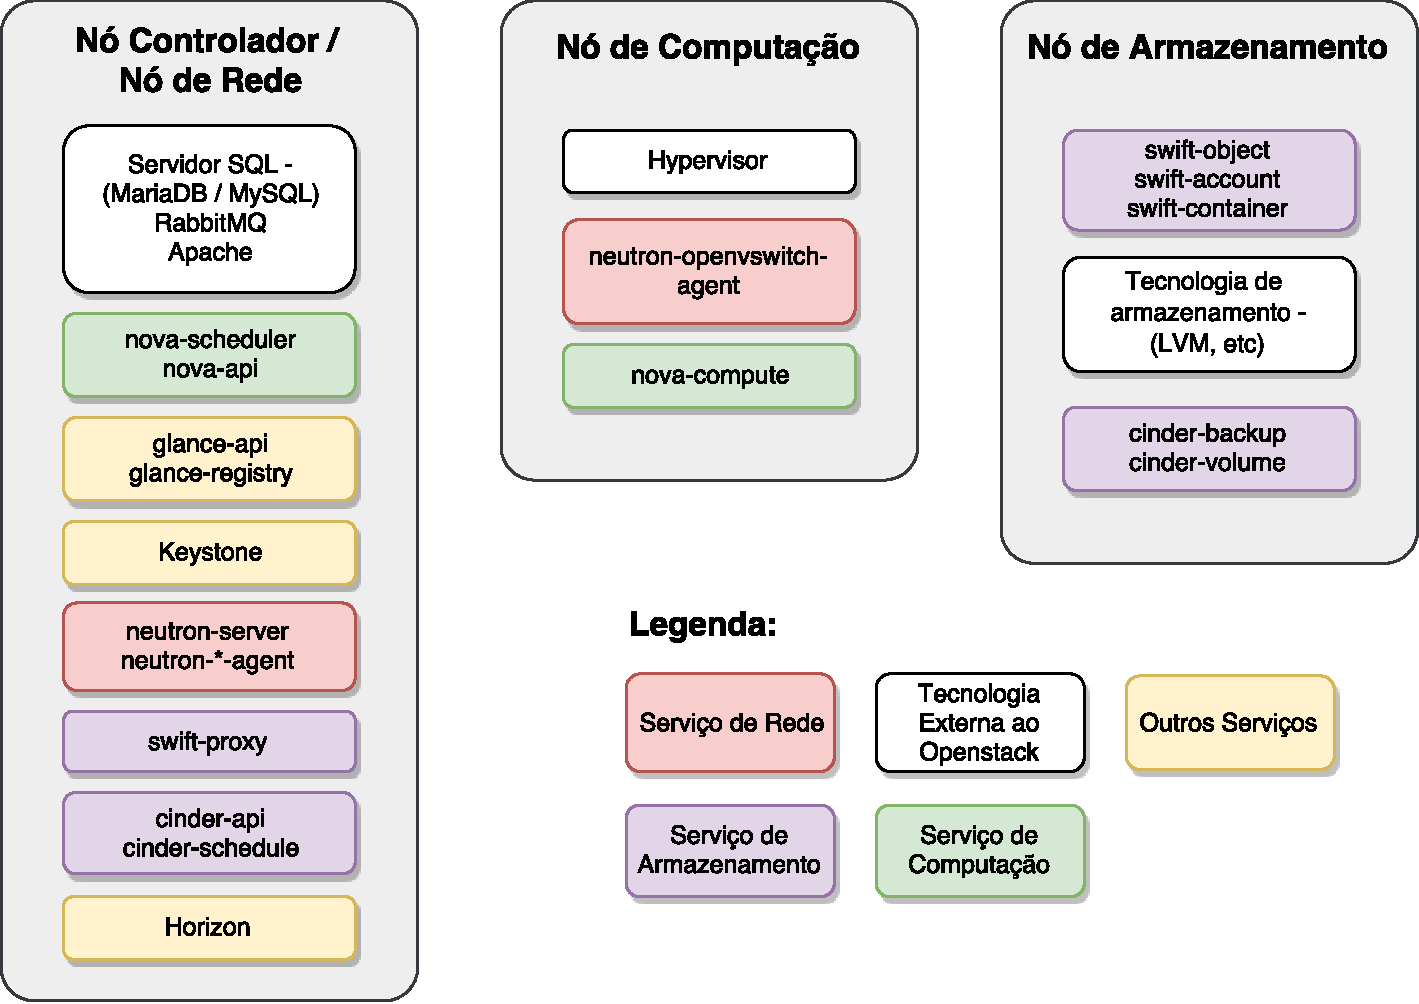
\includegraphics[width=.75\textwidth]{img/openstack_arquitetura_instalacao.pdf}
	\label{fig:openstack_instalacao_servicos}\\
    \vspace{-0.3cm}
	Fonte: O próprio autor.
\end{figure}

\vspace{-0.5cm}
Para explicitar melhor o papel de cada uma das categorias de host no tráfego de controle, esta seção apresenta brevemente como funcionam alguns serviços que executam nestes hosts, com foco na suas respectivas arquiteturas.
%
Os serviços apresentados nesta seção são os considerados no monitoramento e posterior análise do tráfego, conforme definido na Tabela~\ref{tab:openstack_service_list}, com exceção do Horizon, que é basicamente uma interface web que acessa as \acp{api} dos outros serviços, e não será abordado na explicação.
%
Esta limitação de serviços abordados visa simplificar o processo de caracterização, e segue a recomendação de serviços populares em uma instalação do OpenStack, segundo \cite{openstack:about}.



Nem todos os serviços do OpenStack têm a mesma complexidade, e neste sentido, alguns serviços como Nova e Neutron destacam-se pela complexidade.
%
Portanto, nesta seção alguns serviços mais complexos são abordados em mais detalhes do que outros com arquitetura simples (\textit{e.g.,} Keystone, Swift).
%
Além dos serviços, também é apresentada a ferramenta RabbitMQ, que possui papel importante na comunicação entre componentes pertencentes a certos serviços.
%
Esta seção inicia com o Nova, um dos serviços principais no OpenStack, que gerencia o ciclo de vida das \acp{vm} e se relaciona com vários dos serviços do OpenStack para dispor suas funcionalidades (Figura \ref{fig:openstack_service_architecture}).

\subsection{Nova}

O Nova é o serviço de computação do OpenStack, o qual gerencia os nós de computação existentes na nuvem, controlando os \textit{hypervisors} instalados nestes nós, e consequentemente, as \acp{vm} em execução. 
%
Versões anteriores do OpenStack também incluem componentes relacionados à configuração de rede no Nova (\texttt{nova-network}), que disponibiliza um modelo de gerenciamento de rede mais limitado quando comparado ao Neutron, e portanto foi descontinuado.
%
Segundo \citeonline{redhat:components}, as versão recentes do Nova utilizam uma arquitetura que divide-se em diversos componentes, conforme ilustrado na Figura \ref{fig:nova_architecture}.

\begin{figure}[!htb]
	\centering
	\caption{Arquitetura dos componentes pertencentes ao serviço Nova}
    \vspace{-0.3cm}
	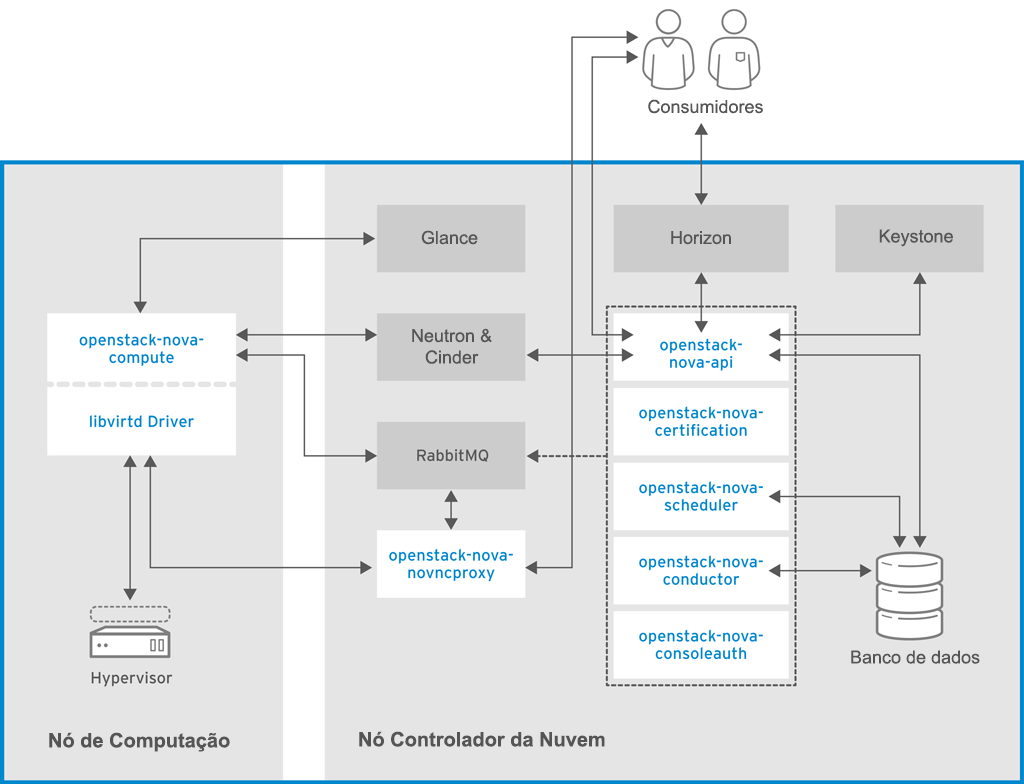
\includegraphics[width=.8\textwidth]{img/nova_arquitetura.png}
	\label{fig:nova_architecture}\\
	Fonte: Adaptado de \cite{redhat:components}.
\end{figure}

Apesar dos vários componentes pertencentes ao serviço Nova (Figura \ref{fig:nova_architecture}), este trabalho foca em alguns componentes principais: \ac{api}, escalonamento, computação, banco de dados, e \textit{message broker} (AMQP Server).

Conforme apresentado na Seção \ref{cap2:openstack}, a \ac{api} do Nova (\texttt{nova-api}) é responsável por disponibilizar acesso e tratar requisições para o serviço Nova.
%
O \texttt{nova-api} em sua essência é um \textit{Web Service} implementado sobre o protocolo REST, e gerencia autorização e funções básicas de controle, na qual implementa modelos de API compatíveis como o da Amazon e Rackspace.
%
Existem diferentes versões da REST \ac{api} do Nova, que introduzem novas funcionalidades ou padronizações, o OpenStack Newton por exemplo, que é a versão que este TCC irá trabalhar, tem a REST \ac{api} do Nova na versão 2.38 \cite{openstack:newton:api}.
%
Toda requisição recebida pelo \texttt{nova-api} é avaliada para verificar se os recursos referenciados na requisição estão disponíveis, e caso estiverem disponíveis, a requisição é enviada ao \textit{message broker}, que é um servidor \acf{amqp}, e disponibiliza a mensagem para os recursos referenciados acessarem \cite{openstack:nova}.
%
O \textit{message broker} é um \textit{middleware} com o protocolo \ac{amqp} utilizado para comunicação interna entre componentes de certos serviços, que no caso do Nova por exemplo, se aplica aos componentes \texttt{nova-scheduler} e \texttt{nova-compute}, e também intermedeia o acesso ao banco de dados pelo \texttt{nova-compute}.

Durante a troca de mensagens, o \textit{message broker} também atualiza o banco de dados do Nova, que mantém informações sobre o estado corrente da nuvem, como por exemplo, o números de \acp{vm} executando em cada nó de computação da nuvem \cite{redhat:components}.
%
Este banco de dados é implementado em MySQL e é acessível pelos componentes do Nova, o qual centraliza as informações que os componentes necessitam durante sua execução.
%
Após receber a mensagem contendo o pedido de \ac{vm} pelo \textit{message broker}, o componente responsável pelo escalonamento, chamado \texttt{nova-scheduler} define qual nó de computação hospedará uma nova instância de \ac{vm}.
%
Para definir o nó de computação é consultado o banco de dados do Nova, que contém informações aplicáveis no processo de filtragem para encontrar um nó de computação disponível para hospedar a \ac{vm}.
%
Neste sentido, é possível fornecer pesos para as métricas, ajudando na escolha do nó de computação, como também é possível deixar a escolha aleatória entre os nós de computação filtrados no processo, que correspondem aos nós de computação podendo hospedar aquela \ac{vm} \cite{openstack:nova}.

No caso de uma nuvem de pequeno porte, os componentes do Nova exibidos até aqui executam em um mesmo nó de controle, pois não necessitam de grande quantidade de processamento.
%
Em contraste, o componente \texttt{nova-compute} executa em cada host que contém um \textit{hypervisor}, ou seja, um nó de computação, e é responsável por gerenciá-los.
%
Como todos os outros componentes do Nova que usam \ac{amqp}, o \texttt{nova-compute} em execução verifica periodicamente por tarefas enfileiradas para ele, e realiza-as conforme solicitado (\textit{e.g.,} criar instância, finalizar instância, ler saída do \textit{console}).
%
Se outros serviços que dispõem funcionalidades extras às \acp{vm} estiverem instalados (\textit{e.g.,} Cinder, Glance, Neutron), cada \texttt{nova-compute} realiza a comunicação direta com estes serviços.


\subsection{Cinder}

Para disponibilizar armazenamento persistente às \acp{vm}, o serviço Cinder permite acoplar volumes/blocos de armazenamento nas \acp{vm} em execução.
%
Além de disponibilizar armazenamento para \acp{vm}, o Cinder também fornece a habilidade de criar \textit{snapshots} dos volumes de armazenamento, que copia o conteúdo do volume, e possibilita gerar novos volumes contendo os dados deste \textit{snapshot}.
%
Mesmo sendo mais simples que o Nova, o Cinder também emprega múltiplos componentes para realizar suas funções, que podem ser distribuídos entre diferentes hosts.
%
Alguns componentes com comportamento similar aos componentes do Nova estão presentes: escalonador, banco de dados, \ac{api} e \textit{message broker}; em que difere-se nos componentes responsáveis pelo armazenamento: \texttt{cinder-backup} e \texttt{cinder-volume}.

O papel do \texttt{cinder-api}, componente que gerencia a \ac{api} do Cinder, é disponibilizar uma interface REST para que os outros serviços do OpenStack, como o Nova, acessem suas funcionalidades \cite{redhat:components}.
%
A REST \ac{api} do Cinder encontra-se na v3.15 no OpenStack Newton \cite{openstack:newton:api}.
%
Após recebido o pedido pelo \texttt{cinder-api}, ele é enviado ao \textit{middleware} responsável pela comunicação entre os componentes, baseado no protocolo \ac{amqp}, e que não necessita ser de uso exclusivo do Cinder.

O banco de dados, baseado em MySQL, tem propósito similar ao banco de dados no Nova: compartilhar informações relacionadas ao estado atual do serviço para os componentes, na qual também pode usar o mesmo servidor de banco de dados.
%
O escalonador \texttt{cinder-scheduler} decide onde armazenar volumes e backups criados, cuja funcionalidade é disponibilizada pelos componentes \texttt{cinder-volume} e \texttt{cinder-backup}, que podem ser hospedados em múltiplos hosts, servindo como nós de armazenamento.
%
Segundo \citeonline{redhat:components}, estes dois componentes podem usar várias soluções de armazenamento (\textit{e.g.,} Ceph, LVM, NFS), e em especial o \texttt{cinder-backup} é capaz de armazenar seus backups no Serviço de armazenamento Swift.

\subsection{Swift}

O Swift é outro serviço do OpenStack responsável pelo armazenamento, mas com o foco em armazenar dados estáticos de grande volume (\textit{e.g.,} vídeos, imagens, imagens de \ac{vm}).
%
O acesso aos dados é feito com o um pedido HTTP (\texttt{Get, Put, Delete}) para o \texttt{swift-proxy}, que é o componente do Swift responsável pela \ac{api}, e autenticação no serviço, que no OpenStack Newton encontra-se na v1 \cite{openstack:newton:api}.
%
Ao receber uma requisição é consultado a localização do objeto nos outros componentes (\texttt{swift-account}, e \texttt{swift-container}, respectivamente), roteando então a requisição de acordo com as informações consultadas, conforme ilustrado na Figura \ref{fig:swift_components}.

O Swift tem dois componentes que gerenciam acesso a listagem de informações: o \texttt{swift-account}, que gerencia a lista de contêineres de armazenamento no banco de dados, e o \texttt{swift-container}, cuja tarefa é gerenciar a lista de objetos contidos nos contêineres, também armazenado no banco de dados.
%
Para gerenciar os objetos armazenados, o componente \texttt{swift-object} armazena, recupera e exclui objetos conforme requisitado \cite{openstack:swift}.
%
A parte de autenticação do \texttt{swift-proxy} comunica-se com o serviço Keystone, que fornece uma \ac{api} que centraliza o processo de autenticação do OpenStack.

\begin{figure}[!htb]
	\centering
	\caption{Arquitetura dos componentes pertencentes ao serviço Swift}
    \vspace{-0.3cm}
	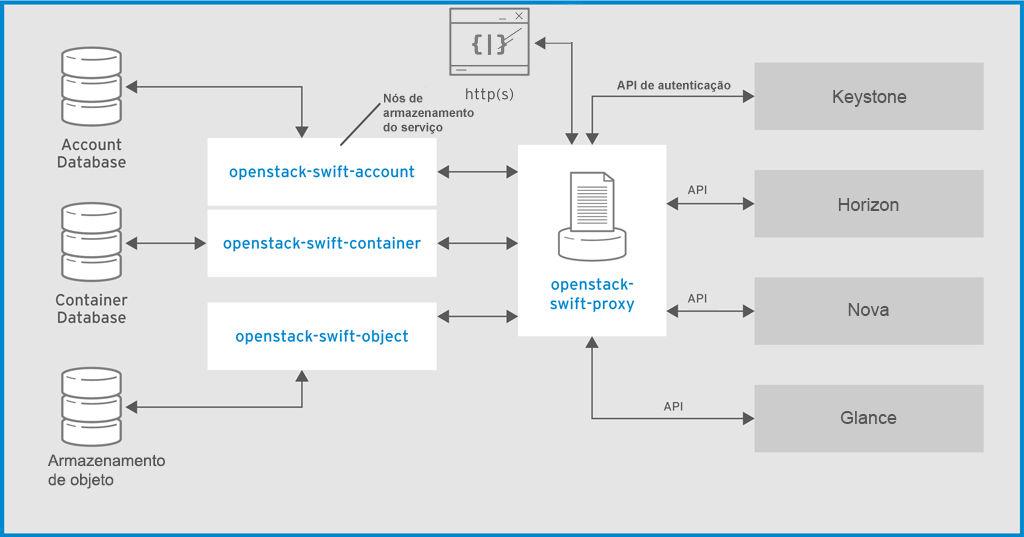
\includegraphics[width=.8\textwidth]{img/swift_arquitetura.png}
	\label{fig:swift_components}\\
	Fonte: Adaptado de \cite{redhat:components}.
\end{figure}

\subsection{Keystone}

O serviço Keystone fornece autenticação e autorização aos serviços do Openstack. 
%
Este serviço possibilita a autenticação através de múltiplos mecanismos, como por exemplo, credencial com usuário e senha, ou através de \textit{tokens} \cite{redhat:components}.
%
Desta maneira, é possível combinar estes mecanismos no uso do Keystone, no qual um pedido de autenticação é validado através de usuário e senha, e então, o serviço pode retornar um \textit{token} ao solicitante, que é utilizado para a autenticação posteriormente \cite{openstack:keystone}.

A arquitetura de funcionamento do Keystone é relativamente simples, possuindo apenas um componente principal, que é responsável pela \ac{api} do serviço, e encontra-se na v3 no OpenStack Newton.
%
A \ac{api} do Keystone armazena as identidades, autorizações, catálogos de serviços e \textit{tokens} no MySQL (MariaDB) por padrão, podendo-se adicionar outras tecnologias para cuidar de partes específicas do serviços. 
%
Neste sentido, a tecnologia \ac{ldap} pode ser empregada no gerenciamento de autenticações e \textit{memcache} ou \textit{Redis} para gerenciar a persistência dos \textit{tokens} \cite{redhat:components}.
%
Após autenticado o usuário (consumidor ou administrador), ele é capaz de acessar o catálogo fornecido pelo Keystone, cuja funcionalidade é armazenar os serviços em funcionamento no Openstack, e informar ao usuário quais recursos ele pode acessar.


\subsection{Glance}

O serviço Glance funciona como um registro de imagens de \acp{vm} acessível pelos consumidores da nuvem. 
%
É possível que os consumidores adicionem novas imagens, desde que estas sejam em um dos formatos aceitos pelo serviço, que segundo \citeonline{redhat:components}, inclui \texttt{iso}, \acp{vm} do VirtualBox (\texttt{vdi}), VMware (\texttt{vmdk}) e Amazon EC2 (\texttt{ami}).
%
Outra alternativa é gerar um \textit{snapshot} a partir de uma das \acp{vm} do consumidor, que pode servir como \textit{backup} ou imagem para iniciar outras \acp{vm}.

Em relação à sua arquitetura, o Glance é dividido nos seguintes componentes principais \cite{openstack:glance}: \texttt{glance-api}, \texttt{glance-registry}, repositório de armazenamento e banco de dados (MySQL/MariaDB).
%
A \ac{api} do Glance (\texttt{glance-api}) gerencia todos os pedidos para recuperação e armazenamento de imagens, que no OpenStack Newton tem a \ac{api} v2 \cite{openstack:newton:api}.
%
Enquanto os pedidos são processados, o componente \texttt{glance-registry} acessa o banco de dados instalado para buscar informações da imagem em questão (\textit{e.g.,} metadados da imagem, local de armazenamento).
%
As imagens registradas neste serviço podem ser armazenadas no serviço Swift ou através de outras tecnologias como RADOS Block Service, VMware datastore, HTTP, ou até como arquivo no próprio sistema de arquivos do host do Glance.


\subsection{Neutron}

Conforme apresentado na Seção \ref{cap2:openstack_network_architecture}, uma das funcionalidades do serviço Neutron é fornecer rede às \acp{vm} dos consumidores, incluindo a possibilidade de configurar a rede em questão, sub-redes e os seus roteadores \cite{redhat:components}.
%
Outras funcionalidades adicionais também podem ser oferecidas para a rede criada em um \textit{project}/\textit{tenant}, como DHCP (\texttt{neutron-dhcp-agent}), \textit{Firewall} ou \acp{vpn}.

\begin{sloppypar}
Comparado com os outros serviços do OpenStack, o Neutron é um dos mais complexos, podendo envolver diversas tecnologias de rede e possibilidades de configuração \cite{denton:2016:neutron}.
%
No geral, o Neutron tem os seguintes componentes: \textit{Network agents}, que inclui os componentes \texttt{neutron-dhcp-agent}, \texttt{neutron-openvswitch-agent} e \texttt{neutron-l3-agent}; \texttt{neutron-server} e \textit{message broker} \cite{openstack:neutron}.
%
Os \textit{Network agents} executam em todos os hosts de uma nuvem OpenStack, e são responsável por cuidar, por exemplo, da configuração das \acp{vm} contidas no host e também de serviços e \textit{plugins} em execução no Neutron, como o Open vSwitch (\texttt{neutron-openvswitch-agent}).
%
O Open vSwitch é uma das tecnologias que pode ser empregada na virtualização das interfaces de rede físicas dos hosts, e permite criar \acp{vlan} para isolar o tráfego de cada rede.
%
Assim, é possível que o tráfego de dois domínios diferentes trafeguem no mesmo meio físico com isolamento.
\end{sloppypar}

O componente \texttt{neutron-ml2} (Modular Layer 2) é obrigatório no Neutron, e controla a Camada 2 da rede, ou seja, encaminha pacote apenas dentro das redes criadas pelos consumidores.
%
A nível estrutural, o \texttt{neutron-ml2} funciona como um \textit{framework} que possibilita a criação de \textit{plugins} que relacionam-se com a Camada 2 da rede, como o TaaS (\textit{Tap-as-a-Service})\footnote{\url{https://github.com/openstack/tap-as-a-service}}, por exemplo.
%
O TaaS possibilita a criação de espelhamentos de portas das redes dos consumidores da nuvem, que tornam-se acessíveis através de portas virtuais criadas pelo TaaS no Open vSwitch, cuja aplicação inclui, por exemplo, o monitoramento do tráfego com um \ac{ids}.
%
Para fornecer acesso à rede externa um \textit{L3 Network agent} (\texttt{neutron-l3-agent}) deve executar no nó de rede da nuvem, e responsabilizar-se pelo roteamento dos pacotes para fora da rede do consumidor, que corresponde à função do roteador virtual inserido pelo consumidor na sua rede \cite{redhat:components}.
%
O agente DHCP (\texttt{neutron-dhcp-agent}) é outro agente que executa no nó de rede, e fornece o serviço de DHCP para as redes dos consumidores.

Por fim, o componente \texttt{neutron-server} é responsável pela \ac{api} do serviço, que age similar aos outros serviços, na qual envia as mensagens para o \textit{message broker}, que encaminha-as para os outros agentes e \textit{plugins} do Neutron.
%
Através da sua \ac{api} os consumidores definem as configurações das suas redes, e o administradores definem as tecnologias de redes empregadas nos serviços do Neutron \cite{denton:2016:neutron}.
%
A \ac{api} do Neutron encontra-se na v2 atualmente, e é a mesma utilizada no OpenStack Newton, na qual baseia-se em um aprimoramento da \ac{api} do Quantum (serviço de rede descontinuado) na v1.1 \cite{openstack:newton:api}.


\subsection{RabbitMQ}

Conforme apresentando nos serviços Neutron, Cinder e Nova, é necessário haver um servidor responsável pela comunicação interna destes serviços, ou seja, entre os seus componentes.
%
O OpenStack emprega o protocolo \ac{amqp} para realizar esta comunicação interna, cujas mensagens são criadas no padrão do protocolo \acf{rpc}, que é implementado pelo projeto Oslo.
%
Neste sentido, o servidor \ac{amqp} (\textit{e.g.,} RabbitMQ, Qpid, ZeroMQ), também chamado de \textit{message broker} apenas transporta a mensagem, seguindo o padrão \textit{publish/subscribe}.
%
A utilização deste \textit{middleware} para comunicação tem como objetivo \cite{openstack:amqp_cinder}: desacoplar o host de origem e destino da mensagem; completo assincronismo entre os hosts (não é necessário que o destino esteja disponível ao enviar mensagem); balanceamento entre chamadas remotas (mensagem é recebida pelo primeiro host disponível a acessar o RabbitMQ). 

Neste meio de comunicação exitem dois tipos de chamadas: \textit{RPC Call} e \textit{RPC Cast} \cite{openstack:amqp_cinder, openstack:amqp_nova}.
%
No \textit{RPC Call}, é enviada uma mensagem do host, e então cria-se um \textit{Consumer} neste host, que escutará a resposta da execução remota, sem efetuar bloqueio no processo de espera.
%
Para saber a quem cada resposta pertence, um campo \texttt{msg\_id} é criado ao enviar a primeira mensagem, e assim o \textit{Publisher} sabe que aquela resposta é para ele.
%
No \textit{RPC Cast}, o método é invocado remotamente, mas sem escutar a resposta de quem o executou.
%
O envio pelo \textit{Publisher} e recebimento de mensagens pelo \textit{Consumer} é separado por tópico, e só os hosts com certo componente ou serviço em execução recebe mensagens de certo tópico.
%
A arquitetura do OpenStack não diferencia os hosts conectados ao RabbitMQ, contudo, é possível verificar uma diferença em comportamento neles, na qual alguns hosts enviam mais mensagens, enquanto outros ficam responsáveis por receber e processar as mensagens.
%
Este tipo de comportamento pode ser verificado ao comparar hosts que executam o \texttt{nova-api} e o \texttt{nova-compute}, por exemplo, em que a \ac{api} repassa tarefas a serem realizadas para outros componentes do Nova, como o \texttt{nova-compute}, que fica à escutar por novas tarefas que deva executar.

\subsection{Considerações OpenStack}
Conhecidos alguns serviços do OpenStack, o próximo passo para a criação do sistema de monitoramento é analisar aspectos específicos de nuvens OpenStack de maneira que auxilie a definir o funcionamento do sistema de monitoramento proposto.
%
Ou seja, objetivo da análise do ambiente de caracterização é definir algumas diretrizes úteis posteriormente: qual é o tráfego de interesse, quais são algumas das características observáveis neste tráfego de interesse, e quais são os locais da rede com maior concentração deste tráfego.

\section{Ambiente de caracterização}
\label{cap3:ambiente}

A Seção \ref{cap3:openstack_detalhes} apresenta a arquitetura de alguns serviços do OpenStack incluídos na caracterizar de tráfego deste TCC.
%
Sendo assim, a partir de suas características de funcionamento podem ser definidas estratégias para criar o sistema de monitoramento responsável por medir o tráfego e o analisar (Seção \ref{cap2:caracterizacao}).
%
O propósito desta seção é exibir características do OpenStack apresentadas neste TCC que podem ser exploradas na construção do sistema de monitoramento.

As \acp{api} dos serviços do OpenStack são responsáveis por expor suas funcionalidades aos consumidores da nuvem e a outros serviços.
%
Neste sentido, toda ação realizada na nuvem por algum consumidor inicia-se através da comunicação com a \ac{api}.
%
Após a realização de um pedido através da \ac{api}, o serviço correspondente retorna uma mensagem informando sobre o \textit{status} da ação realizada (\textit{e.g.,} sucesso, falha, informações à respeito).
%
Logo, é possível descobrir se o consumidor foi capaz de realizar certa ação ao olhar a resposta recebida.
%
Sendo assim, monitorar as mensagens que passam pelas \acp{api} em busca de comportamentos de interesse é uma maneira de entender o que ocorre na nuvem.
%
A Figura \ref{code:nova_api_response} apresenta uma resposta ao realizar uma consulta para a \ac{api} do Nova (\texttt{nova-compute}) solicitando a lista de volumes fornecidos pelo Cinder que estão acoplados em uma certa \ac{vm}.

\begin{figure}[!htb]
	\centering
    \caption{Exemplo de resposta recebida ao consultar volumes de armazenamento acoplados a uma instância do Nova}
    \begin{minted}{json}
{
    "volumeAttachments": [
        {
            "device": "/dev/sdd",
            "id": "a26887c6-c47b-4654-abb5-dfadf7d3f803",
            "serverId": "4d8c3732-a248-40ed-bebc-539a6ffd25c0",
            "volumeId": "a26887c6-c47b-4654-abb5-dfadf7d3f803"
        },
        {
            "device": "/dev/sdc",
            "id": "a26887c6-c47b-4654-abb5-dfadf7d3f804",
            "serverId": "4d8c3732-a248-40ed-bebc-539a6ffd25c0",
            "volumeId": "a26887c6-c47b-4654-abb5-dfadf7d3f804"
        }
    ]
}
	\end{minted}
    \label{code:nova_api_response}
    Fonte: \cite{openstack:nova_api_response}.
\end{figure}

A resposta segue o padrão REST, e é formatado com JSON, na qual pode-se aplicar ferramentas de \textit{parse} ou análise com expressão regular para extrair informações.
%
No caso de falha, por exemplo, esta mensagem no protocolo HTTP poderia retornar algum código de erro, como o código 401 (\texttt{unathorized}) caso o solicitante não tenha permissão para acessar a informação \cite{openstack:nova_api_response}.

A partir do monitoramento da \ac{api} é possível visualizar a requisição de uma ação na nuvem e a resposta resultante do sistema.
%
Ou seja, enxerga-se a nuvem como uma caixa preta, observando a entrada e a saída resultante da \ac{api}.
%
Para aumentar a quantidade de informações disponíveis, é possível observar o conteúdo desta ``caixa preta'' através do monitoramento da comunicação entre componentes de um serviço.

Serviços complexos como o Nova, Neutron e Cinder possuem componentes distribuídos pela nuvem, e a responsabilidade da comunicação entre estes componentes fica a cargo do \textit{middleware} de comunicação (RabbitMQ).
%
Conforme apresentado na Seção \ref{cap3:openstack_detalhes}, quando um componente de algum serviço como o Nova enviar uma mensagem \ac{rpc} para o RabbitMQ, a mensagem é recebida por um componente com interesse nela (tópico da mensagem).
%
Contudo, uma mensagem enviada para o RabbitMQ pode esperar certo tempo até ser recebida por algum destino, pois algum dos destinos em potencial deve verificar se há alguma mensagem de interesse disponível para receber do \textit{middleware} de comunicação.
%
Sendo assim, ao monitorar as mensagens \textbf{saindo} do RabbitMQ pode-se ter certeza que aquelas mensagens serão processadas logo em seguida pelo destino.

O sistema de monitoramento de \cite{sharma:2015:hansel} analisa o tráfego \ac{rpc} e REST, com o objetivo de organizá-lo numa sequência de mensagens que representa um evento na nuvem.
%
A sequência é criada ao encontrar várias mensagens com o mesmo identificador, que segundo \cite{sharma:2015:hansel}, o OpenStack utiliza para controle interno.
%
Portanto, é possível relacionar requisições dos consumidores da nuvem e as subsequentes comunicações entre os componentes para executá-las.
%
Porém, uma dificuldade encontrada por \cite{sharma:2015:hansel} ao analisar mensagens \ac{rpc} é a ausência de uma maneira simples de indicar a presença de erro.
%
Uma estratégia de uso para empregar ambos os protocolos pode consistir da análise de mensagens REST em direção à \ac{api}, e então de acordo com o tipo de ação, caso houver necessidade de acompanhar o processo detalhadamente, pode-se analisar o tráfego RPC gerado em função desta requisição REST.

Serviços do OpenStack executam por padrão na rede de controle com as portas definidas segundo a Tabela \ref{tab:openstack_service_list}, e não mudam durante a execução.
%
Logo, é possível associar cada pacote de controle na nuvem ao serviço do OpenStack de destino através da porta de destino definida no cabeçalho do pacote.
%
Mesmo este método de classificação sendo simples, com ele é possível realizar uma medição que classifica, por exemplo, os serviços do OpenStack que recebem mais mensagens.
%
Contudo, para garantir que a classificação apresente resultados significativos é necessário isolar o tráfego de armazenamento.
%
A justificativa é que a transferência de uma imagem de \acp{vm} ou de um volume de armazenamento, por exemplo, é feita com vários pacotes, podendo impactar significativamente a medição realizada.

Em relação ao processo de coleta de tráfego, ou seja, na fase de medição do tráfego da rede de controle, é necessário que a abordagem meça o tráfego gerado pelo OpenStack.
%
Com isso em mente, a medição ativa possui pouca aplicabilidade, pois o princípio desta abordagem é justamente depender apenas do tráfego gerado pelo próprio software de monitoramento, descartando a necessidade de conhecer características da rede (\textit{e.g.,} topologia, comportamento) cuja medição será realizada.
%
Portanto, no caso da rede de controle de uma nuvem OpenStack, por exemplo, a medição de tráfego passiva é a melhor escolha, visto que diferente da abordagem ativa, a medição passiva coleta todo o tráfego no ponto de medição, que na rede de controle é gerado apenas pelo OpenStack e tecnologias relacionadas.

Escolhida a abordagem de medição passiva, o próximo passo é decidir sobre o ponto de medição, que pode ser distribuído em vários pontos da rede dependendo da necessidade.
%
Considerando o que foi apresentado sobre o tráfego \ac{rpc} e REST no começo desta seção, por exemplo, deve-se escolher um ou mais pontos de coleta de maneira que a medição cubra o máximo de tráfego de interesse quanto possível (\textit{e.g.,} mensagens em \ac{rpc} e REST).
%
Neste sentido, conforme ilustrado na Figura \ref{fig:openstack_instalacao_servicos}, os serviços do OpenStack e outras tecnologias relacionadas com as \acp{api} e comunicação interna de serviços (\textit{e.g.,} RabbitMQ) são distribuídas entre nós de rede e de controle da nuvem.
%
Logo, os nós de rede e de controle de uma nuvem OpenStack são potencialmente bons locais para posicionar a parte responsável pela medição de tráfego no sistema de monitoramento.
%
%Definidas algumas das abordagens possíveis para monitorar o tráfego com base nas características observadas, a Seção \ref{cap3:monitoramento} aplica algumas destas informações na criação do sistema de monitoramento.


\section{Especificação de requisitos}
\label{cap3:requisitos}

Com o objetivo de solucionar o problema de caracterização de tráfego, abordado na Seção \ref{cap2:problema}, esta seção inicia a proposta de solução apresentando alguns requisitos que devem ser considerados na proposta.
%
Estes requisitos estão associados à primeira parte do processo de caracterização de tráfego proposto, que é a medição de tráfego, e que será de responsabilidade do sistema de monitoramento.
%
Sendo assim, existem pré-requisitos para possibilitar que o sistema de monitoramento realize a medição de tráfego corretamente:

\begin{itemize}
	\item Ter acesso ao tráfego que passa pelas interfaces de rede, físicas e virtuais, da nuvem monitorada;
    %\item O dispositivo monitorado deve ter memória suficiente disponível;
    \item Um dispositivo de monitoramento necessita estar conectado à rede de controle da nuvem que pertence; e
    \item Existir um banco de dados de dados acessível para armazenar os dados gerados.
\end{itemize}

Os requisitos são abstrações de funcionalidades que monitoram aspectos observáveis na rede de controle.
%
Estes aspectos monitorados serão consultados na fase de análise do tráfego.
%
Os requisitos que devem possibilitar a medição do tráfego da rede de controle, a fim de gerar informações sobre aspectos observáveis do tráfego são divididos em requisitos funcionais e requisitos não funcionais:

Requisitos funcionais:
\begin{itemize}
	\item \textbf{RF1.} Contabilizar o consumo de tráfego na rede de controle dos serviços em execução;
    \item \textbf{RF2.} Armazenar a comunicação entre os componentes dos serviços em execução;
    \item \textbf{RF3.} Armazenar as requisições recebidas pelas \acp{api}, originárias tanto de consumidores quanto de outros serviços; e
    \item \textbf{RF4.} Os dados devem ser detalhados, de maneira que eles revelem tarefas responsáveis por variações na nuvem.
\end{itemize}

Requisitos não funcionais:
\begin{itemize}
	\item \textbf{RNF1.} Operar independente do OpenStack, não sendo atrelado a uma implementação de nuvem apenas; e
    %\item Ser fácil de implementar;
    \item \textbf{RNF2.} O sistema de monitoramento não pode impactar no desempenho da nuvem sendo analisada.
\end{itemize}


\section{Proposta de sistema de monitoramento}
\label{cap3:monitoramento}

Definido o tráfego de interesse, como obter este tráfego (Seção \ref{cap3:ambiente}), e os requisitos do sistema de monitoramento (Seção \ref{cap3:requisitos}), o próximo passo é estipular a arquitetura do sistema de monitoramento que auxiliará na caracterização de tráfego da rede de controle.
%
A princípio, este sistema de monitoramento terá três funcionalidades, que são baseadas nos requisitos funcionais especificados:

\begin{itemize}
  \item \textbf{F1.} Analisar o consumo de banda na rede de controle, classificando em função do serviço que receberá o tráfego (RF1);
  \item \textbf{F2.} Registrar requisições nas \acp{api} dos serviços, que originam tanto de outros serviços como de consumidores (RF3); e
  \item \textbf{F3.} Registrar transações internas da nuvem, que trafegam pelo \textit{middleware} de comunicação (RabbitMQ) (RF2).
\end{itemize}

As funcionalidades devem coletar o tráfego de controle através da medição passiva. 
%
Portanto, instâncias do sistema de monitoramento executarão em cada um dos hosts de interesse (pontos de medição escolhidos explicado na Seção \ref{cap3:ambiente}), conforme ilustrado na Figura \ref{fig:proposta_instalacao}.

\begin{figure}[!htb]
	\centering
	\caption{Arquitetura de instalação do sistema de monitoramento}
    \vspace{-0.5cm}
	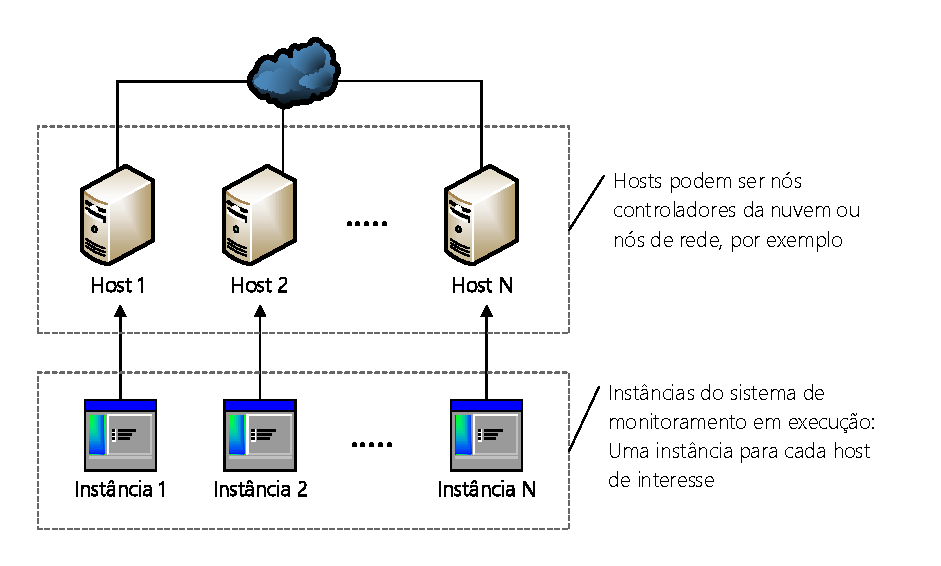
\includegraphics[width=.9\textwidth]{img/arquitetura_instalacao.pdf}
	\label{fig:proposta_instalacao}\\
    \vspace{-0.3cm}
	Fonte: O próprio autor.
\end{figure}

Apesar de nem todos os hosts hospedarem \acp{api} dos serviços (F2) ou o RabbitMQ (F3), pode haver interesse em monitorar tal host caso o tráfego de controle de algum serviço de interesse origine ou vá para ele (F1).
%
A decisão se o pacote está relacionado com algum serviço de interesse é baseada na porta de destino, seguindo as portas por padrão na Tabela \ref{tab:openstack_service_list}.
%
Para realizar a coleta de tráfego, este sistema de monitoramento será desenvolvido em uma linguagem de alto nível que forneça métodos relacionados à biblioteca \texttt{libpcap}.
%
Esta biblioteca disponibiliza meios para sistemas UNIX capturarem tráfego em suas interfaces de rede, sendo elas virtuais ou físicas.
%
Das linguagens possíveis, a preferência é para Python, por dispor de diversas bibliotecas e funcionalidades que simplificam o desenvolvimento, mas podendo mudar caso desempenho torne-se um fator crítico, seguindo o requisito RNF2.

Abordando o comportamento do sistema em alto nível é possível abstrair comportamentos comuns às três funcionalidades, conforme ilustrado na Figura~\ref{fig:proposta_funcionamento}.
%
\begin{figure}[!htb]
	\centering
	\caption{Arquitetura do sistema de monitoramento em alto nível}
    \vspace{-0.5cm}
	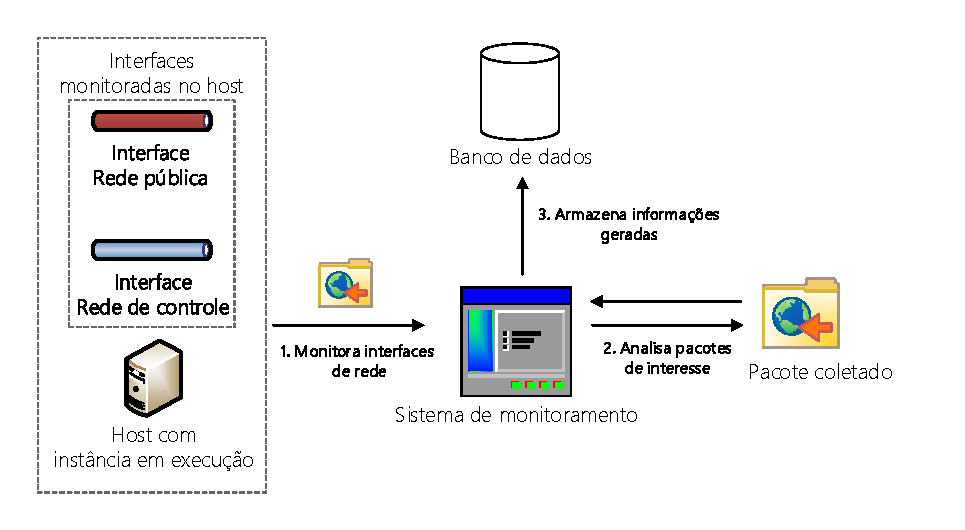
\includegraphics[width=1\textwidth]{img/arquitetura_funcionamento.pdf}
	\label{fig:proposta_funcionamento}\\
    \vspace{-0.6cm}
	Fonte: O próprio autor.
\end{figure}

\vspace{-0.3cm}
O sistema de monitoramento executará em um host de interesse, coletando tráfego nas interfaces de rede de acordo com as funcionalidades do sistema de monitoramento em execução naquele host, respeitando o requisito RNF1 (passo 1 na Figura \ref{fig:proposta_funcionamento}).
%
Caso um host não hospede \acp{api} de serviços, ou o \textit{middleware} de comunicação, por exemplo, é possível executar o sistema de monitoramento apenas para monitorar o tráfego na interface da rede de controle, pois é por onde passa o tráfego dos serviços de interesse, que é registrado pela F1.
%
Apesar de existirem outros níveis de agregação de tráfego, neste sistema de monitoramento é necessário realizar a medição a nível de pacote.
%
A agregação a nível de fluxo, por exemplo, apesar de popular, omite detalhes relevantes para este sistema de monitoramento, como o conteúdo do pacote.
%
Outro motivo é que apenas um pacote pode ser o suficiente para provocar mudanças no comportamento da nuvem, tal como uma requisição de criação de instância.
%
A agregação de tráfego com uma granularidade mais grossa perde tais detalhes, que devem ser levados em consideração no monitoramento, de acordo com o requisito RF4.

Os pacotes coletados são filtrados conforme a funcionalidade em execução no sistema de monitoramento daquele host, que nos três casos verificam a porta de destino (passo 2 na Figura \ref{fig:proposta_funcionamento}).
%
Na F1, qualquer pacote que tenha a porta de destino pertencente a uma das portas contida na Tabela \ref{tab:openstack_service_list}, por padrão, será aceito.
%
Em relação à F2, apenas pacotes destinados às portas na qual as \acp{api} executam serão aceitos.
%
Para a F3, os pacotes destinados à porta na qual o RabbitMQ executa serão aceitos.
%
Após, cada funcionalidade realiza seu processamento utilizado informações extraídas dos pacotes filtrados, posteriormente gravando no banco de dados escolhido, que é acessado por todas as instâncias em execução para gravar as informações geradas (passo 3 na Figura \ref{fig:proposta_funcionamento}).
%
Em relação aos dados armazenados, cada funcionalidade terá sua própria estrutura de armazenamento no banco de dados, que no caso de banco de dados relacionais (\textit{i.e.,} MySQL, PostgreSQL), é o equivalente a uma ou mais tabelas para cada funcionalidade.
%
O restante desta seção detalhará o funcionamento das três funcionalidades de monitoramento, na qual F2 e F3 serão agrupadas na explicação por conta da sua semelhança no funcionamento.

\subsection{F1: Classificação consumo de banda, rede de controle}
% @TODO -> parei revisão 1 aqui
Esta funcionalidade tem como objetivo auxiliar na análise longitudinal de tráfego na rede de controle.
%
Contudo, será considerado apenas o tráfego gerado pelos serviços delimitados na Tabela~\ref{tab:openstack_service_list} para simplificar o escopo deste TCC.
%
O diagrama de sequência na Figura \ref{fig:proposta_sequencia_servicos} ilustra os passos de funcionamento desta funcionalidade do sistema de monitoramento.

\begin{figure}[!htb]
	\centering
	\caption{Diagrama de sequência: monitoramento de banda consumida pelos serviços}
    \vspace{-0.3cm}
	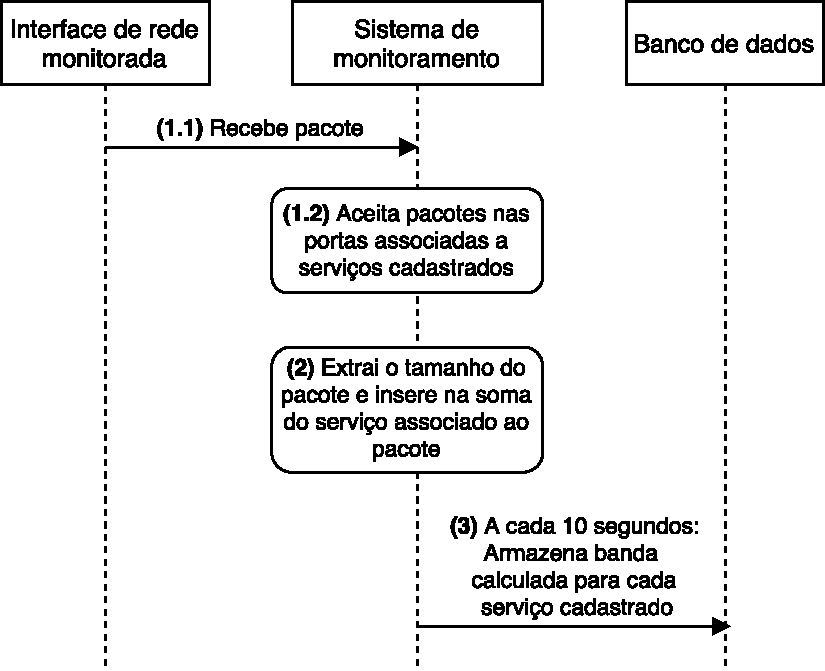
\includegraphics[width=0.77\textwidth]{img/sequencia_monitoramentoServicos.pdf}
	\label{fig:proposta_sequencia_servicos}\\
%    \vspace{-0.3cm}
	Fonte: O próprio autor.
\end{figure}

Os passos que esta funcionalidade executa são:

\begin{enumerate}
\item Esta funcionalidade monitora apenas a interface da rede de controle, buscando todo tráfego que tenha como destino uma das portas associadas aos serviços em execução naquele host.
%
As portas também são utilizadas para criar uma classificação de serviços, cuja porta de destino serve para decidir em qual serviço aquele pacote está associado;

\item Após definido o serviço destino daquele pacote, é extraído o tamanho daquele pacote, que é somado a um contador de tráfego para aquele serviço.
%
Assim, por exemplo, todos os pacotes recebidos por certo serviço ao longo de um tempo têm seu tamanho somado, e então esta soma é dividida pelo período de tempo estabelecido (\textit{e.g.,} 5s, 10s).
%
Ou seja, ao somar todo o tráfego recebido ao longo de um período, e depois dividir esta soma pelo período, é possível estabelecer uma aproximação da quantidade de banda utilizada (em KB/s) para o serviço em questão naquele período.
%
Esta técnica é feita para todos os serviços considerados nesta análise, cada qual tendo seu próprio contador; e

\item Para cada uma destas somas é feita uma entrada no banco de dados, contendo o serviço e o cálculo de banda usada pelo serviço.
%
No caso de oito serviços monitorados com um período de 10s, por exemplo, a cada 10s serão realizadas oito inserções, em que cada uma contém a quantidade de banda destinada ao seu serviço naqueles 10s.
%
Após realizada a inserção o contador de cada serviço volta para zero, e faz o processo de inserção no banco de dados após 10s novamente.
\end{enumerate}


\subsection{F2 e F3: Cadastrar eventos detectados na \ac{api} dos serviços e no \textit{middleware} de comunicação}

Ambas F2 e F3 comportam-se de maneira similar, variando apenas a porta de destino observada e o conteúdo/protocolo dos pacotes analisados.
%
A Figura~\ref{fig:proposta_sequencia_transacao} ilustra um diagrama de sequência para F3, que monitora as transações internas da nuvem passando pelo \textit{middleware} de comunicação.
%
Para gerar informações significativas deve-se relacionar os dados gerados por estas funcionalidades com outras, sendo possível relacionar as duas, por exemplo, e criar uma sequência detalhada de ações na nuvem a partir de uma requisição, conforme feito por \citeonline{sharma:2015:hansel}.

\begin{figure}[!htb]
	\centering
	\caption{Diagrama de sequência: monitoramento de transações internas da nuvem}
	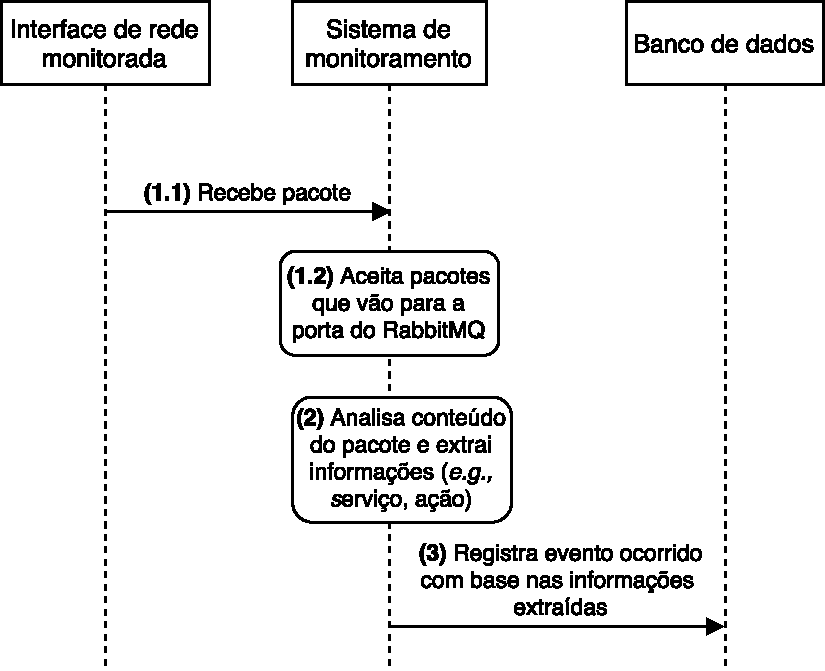
\includegraphics[width=0.78\textwidth]{img/sequencia_monitoramentoTarefas.pdf}
	\label{fig:proposta_sequencia_transacao}\\
	Fonte: O próprio autor.
\end{figure}

As ações nestas funcionalidades ocorrem da seguinte forma, tomando o diagrama de sequência da F3 (Figura \ref{fig:proposta_sequencia_transacao}) como base:

\begin{enumerate}
\item A F2 monitora a interface da rede pública, enquanto a F3 monitora a interface da rede de controle.
%
Ao receber pacotes, ambas as funcionalidades olham na porta de destino para decidir se aceitam os pacotes, na qual a F2 verifica se a porta de destino é de uma \ac{api} que o host hospeda; e no caso da F3, é verificado se a porta de destino é a mesma que a do \textit{middleware} de comunicação que o host hospeda; e

\item A princípio ambas as funcionalidades armazenarão as mesmas informações, mesmo que os protocolos de comunicação analisados sejam diferentes (HTTP na F2, e \ac{rpc} na F3).
%
Ou seja, para ambos as principais informações a armazenar são: serviço de origem, serviço de destino, IP do host e identificador da ação;

\item Por fim, armazena-se os dados de cada funcionalidade em suas respectivas tabelas.
\end{enumerate}


Conforme definido, através da implementação deste sistema de monitoramento será possível gerar os dados necessários para realizar a caracterização de tráfego proposta para a rede de controle.
%
A F1 é capaz de gerar informações relevantes em tempo real, possibilitando, por exemplo, verificar a variação do uso de banda pelos serviços ao longo de um período determinado.
%
Diferentemente, as funcionalidades F2 e F3 geram dados que necessitam de uma análise mais minuciosa, realizada na etapa posterior à coleta, especificada na Seção \ref{cap3:analise}.


\section{Análise de tráfego}
\label{cap3:analise}

A etapa de análise de tráfego, que será aplicada nos dados gerados pelo sistema de monitoramento (definido na Seção \ref{cap3:monitoramento}) busca gerar informações que ajudem a compreender melhor o comportamento do tráfego analisado.
%
Esta análise terá escopo limitado, no sentido de considerar apenas os serviços contidos na implementação mais popular de nuvem OpenStack, segundo \citeonline{openstack:newton}: Nova, Neutron, Cinder, Swift, Keystone e Glance.
%
A proposta atual pretende caracterizar três ângulos diferentes na rede de controle:

\begin{itemize}
	\item \textbf{Caracterização de funcionalidades da nuvem:} Busca entender como a execução de tarefas pelo consumidor influencia no funcionamento da rede de Controle da nuvem. 
	%
	A proposta inicial tem foco no ciclo de vida de \acp{vm} do OpenStack (\textit{e.g.,} criação de \ac{vm}, iniciação de \ac{vm}, pausar \ac{vm} em execução).
	
	\item \textbf{Consumo de banda por serviços:} Esta análise longitudinal tem como objetivo entender quais dos serviços considerados na análise mais geram tráfego na rede de Controle.
	
	\item \textbf{Influência de eventos periódicos no comportamento da nuvem:} Listar alguns dos eventos periódicos gerados pelos serviços da nuvem, e verificar qual o impacto gerado por eles na rede de controle. 
\end{itemize}

A \textbf{caracterização de funcionalidades da nuvem} utilizará informações geradas pelas F2 e F3, definidas no sistema de monitoramento.
%
Estas funcionalidades geram dados referentes à comunicação com as \acp{api} da nuvem, e da comunicação interna dos serviços, feita através do RabbitMQ.
%
Sendo assim, é possível criar uma sequência que mostra a trajetória do tráfego durante a realização de uma tarefa na nuvem a partir de uma requisição recebida pela \ac{api}.
%
Ou seja, a partir de uma requisição de um consumidor (\textit{e.g., } criação de \ac{vm}), cria-se um grafo direcionado que mostra quais mensagens foram enviadas para quais serviços à fim de concretizar a tarefa em questão.
%
Segundo \cite{sharma:2015:hansel} é possível gerar esta sequência de eventos, mas ainda não foi realizada uma análise profunda para verificar se realmente existe alguma variável que pode ser utilizada para interligar estas mensagens diretamente.

A análise de \textbf{consumo de banda por serviços} baseia-se na F1 do sistema de monitoramento, que contabiliza o tráfego gerado por cada um dos serviços considerados na análise.
%
A F1 do sistema de monitoramento deve gerar dados que podem ser interpretados diretamente, possibilitando a realização desta análise em tempo real.
%
Sendo assim, é possível por exemplo, acessar os dados gerados por esta funcionalidade definindo o período de início e de fim da análise, na qual gera um gráfico mostrando qual a porcentagem de tráfego destinado a cada serviço.

Por fim, a análise da \textbf{influência de eventos periódicos no comportamento da nuvem} deve se basear principalmente nos dados gerados pela F1 do sistema de monitoramento, na qual buscará grandes variações no recebimento de tráfego dos serviços em curtos períodos de tempo.
%
Baseando-se nestas variações serão consultados os dados gerados pelas F2 e F3 naquele período, que constará quais serviços enviaram as mensagens em questão.
%
Ou seja, como produto final este ângulo de caracterização busca mostrar quem executou aquele evento periódico, qual a tarefa em questão, e se há impacto significativo.
%
Definida a abordagem utilizada para a realização da caracterização de tráfego, o passo final é explicar como será realizado o experimento que aplicará a proposta definida neste capítulo.


\section{Plano de testes}
\label{cap3:experimento}

O plano de testes visa definir os experimentos a serem executados, os quais aplicarão a proposta de caracterização de tráfego.
%
A finalidade destes experimentos é validar o sistema de monitoramento desenvolvido e a abordagem para análise do tráfego.
%
No total serão realizados três experimentos, divididos em dois cenários diferentes, sendo que dois experimentos serão realizados em um dos cenários, e o outro cenário será usado no experimento restante.

\begin{itemize}
\item \textbf{Cenário 1:} Uma nuvem OpenStack com ambiente controlado, na qual toda interação com ela será originária dos experimentos executados; e

\item \textbf{Cenário 2:} Uma nuvem OpenStack em ambiente de produção, com consumidores utilizando-a.
\end{itemize}

Os experimentos visam verificar o funcionamento do sistema de monitoramento, e então analisar os dados gerados após a execução. 
%
Estes experimentos são:

\iffalse
\begin{itemize}
	\item \textbf{Experimento 1:} Visa verificar o funcionamento da função do sistema de monitoramento responsável por registrar o consumo de banda na rede de controle dos serviços do OpenStack, que será realizado no \textbf{cenário 1}.
    %
    O sistema de monitoramento executará apenas a função responsável por registrar o consumo de banda dos serviços, na qual o período de monitoramento será de um dia.
    %
    Durante este período, a nuvem em questão não receberá qualquer requisição originária de consumidor, e não hospedará nenhuma \ac{vm} em execução.
    %
    Os dados de consumo de banda gerados neste experimento serão armazenados e analisados, com o objetivo de estabelecer uma linha base de consumo de banda em nuvens OpenStack.
\end{itemize}
\fi

\begin{itemize}
	\item \textbf{Experimento 1:} Verificar o funcionamento do sistema de monitoramento, com o objetivo de avaliar a quantidade de dados gerados no monitoramento do \textbf{Cenário 1}.
    %
    O sistema de monitoramento utilizará todos as suas funcionalidades, na qual instâncias executarão em todos os hosts de interesse por um período de sete dias.
    %
    Durante este período, a nuvem deverá receber algumas requisições, que simularão atividades de consumidores, mas de forma esporádica.
    %
    Deste modo, será avaliada a quantidade de dados gerados, com o objetivo de verificar, por exemplo, se o banco de dados utilizado é adequado no caso de monitorar uma nuvem em ambiente de produção.
\end{itemize}

\begin{itemize}
	\item \textbf{Experimento 2:} Análise longitudinal do consumo de banda pelos serviços de uma nuvem em ambiente de produção (\textbf{Cenário 2}).
    %
    A função que registra o consumo de banda pelos serviços do OpenStack executará por um período de 30 dias.
    %
    Após, com os dados coletados será feita uma análise, com o objetivo de verificar a variação do consumo ao longo do período, identificando padrões de comportamento, por exemplo.
\end{itemize}

\begin{itemize}
	\item \textbf{Experimento 3:} Caracterização do comportamento da rede de controle em uma nuvem em ambiente de produção (\textbf{Cenário 2}).
    %
    O sistema de monitoramento utilizará todas as suas funcionalidades, na qual instâncias executarão em todos os hosts de interesse por um período de sete dias.
    %
    Ao longo deste período, a nuvem em questão será usada pelos consumidores e o sistema de monitoramento irá gerar dados sobre o uso.
    %
    Após, será feita uma caracterização de tráfego abordando dois ângulos de análise, definidos na Seção \ref{cap3:analise}: influência de eventos periódicos no comportamento da nuvem, e caracterização de funcionalidades da nuvem.
\end{itemize}

	Como comparativo, serão avaliados o tamanho do banco de dados nos experimentos 1 e 3, e verificar se há grande mudança na quantidade de dados gerados a partir do monitoramento.
    %
    Ambos os cenários utilizarão uma instalação similar do OpenStack, na qual os serviços caracterizados serão os mesmos.
    
    
\section{Considerações do Capítulo}
\label{cap3:consideracoes}

Este capítulo apresentou a proposta de caracterização de tráfego para uma nuvem computacional OpenStack.
%
A proposta baseia-se na análise da arquitetura de funcionamento de alguns serviços do OpenStack, o que possibilitou a definição de estratégias para utilizar no sistema de monitoramento, responsável pela primeira etapa: a medição de tráfego.
%
Foram definidos requisitos para a criação deste sistema de monitoramento, que abordam suas funcionalidades, e também pré requisitos, que devem ser considerados na construção dele.
%
O sistema de monitoramento em questão terá três funcionalidades que irão medir o tráfego e popular um banco de dados com as informações geradas a partir do tráfego avaliado.
%
Então, a etapa posterior, de análise de tráfego utilizará estas informações para melhor entender o comportamento da rede de controle sobre três ângulos de análise diferentes.
%
Após definir o que deve ser feito, a especificação do plano de testes determinou quais os experimentos que serão realizados, e também estabeleceu os cenários empregados nos experimentos.